% Título de la Parte
\section{LABORATORIOS CON SOFTWARE}
\begin{frame}

\pgfdeclareimage[width=\paperwidth,height=\paperheight]{bg}{imagenes/fondo_seccion}
\setbeamertemplate{background}{\pgfuseimage{bg}}

\definecolor{greenU}{RGB}{212,202,72}
\setbeamercolor{block body}{fg=Black,bg=greenU}
\begin{block}{}
\centering
\vspace{8mm}
%% Se repite título de la sección
\Large{LABORATORIOS CON SOFTWARE}
\vspace{8mm}
\end{block}
\end{frame}
%-----------------------

{
\begin{frame}
\frametitle{Parte I - Tabla de contenidos}
\begin{spacing}{1.5}
% genera la tabla de contenidos	
\tableofcontents[currentsection,sectionstyle=hide/hide,subsectionstyle=show/show/hide, subsubsectionstyle=hide]
\end{spacing}
\end{frame}
}

% se incluyen los laboratorios pertenecientes a la Parte

%///////////////////////////////////////////////////////////////

\subsection{Lab1: Primeros pasos}
%*********************
\begin{frame}{}

\pgfdeclareimage[width=\paperwidth,height=\paperheight]{bg}{imagenes/fondo_lab}
\setbeamertemplate{background}{\pgfuseimage{bg}}

\bfseries{\textrm{\LARGE Lab1\\ \Large Primeros pasos}}
\raggedright
\end{frame}
%*********************

\begin{frame}{Primeros pasos}

\pgfdeclareimage[width=\paperwidth,height=\paperheight]{bg}{imagenes/fondo3}
\setbeamertemplate{background}{\pgfuseimage{bg}}

\begin{figure}[H]
\centering
\vspace{-3mm}
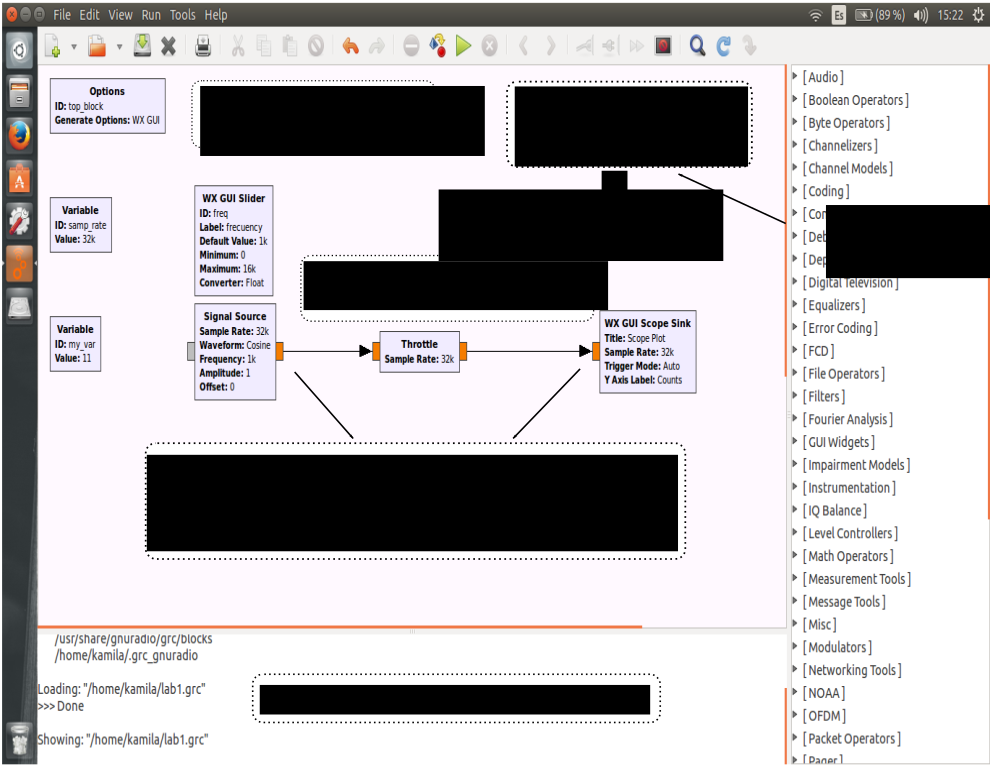
\includegraphics[width=0.9\textwidth]{parte1/lab1/pdf/lab1_1.pdf}
\end{figure}
\end{frame}
%-----------------------------------

\begin{frame}{Primeros pasos }
\begin{figure}[H]
\centering
\vspace{-3mm}
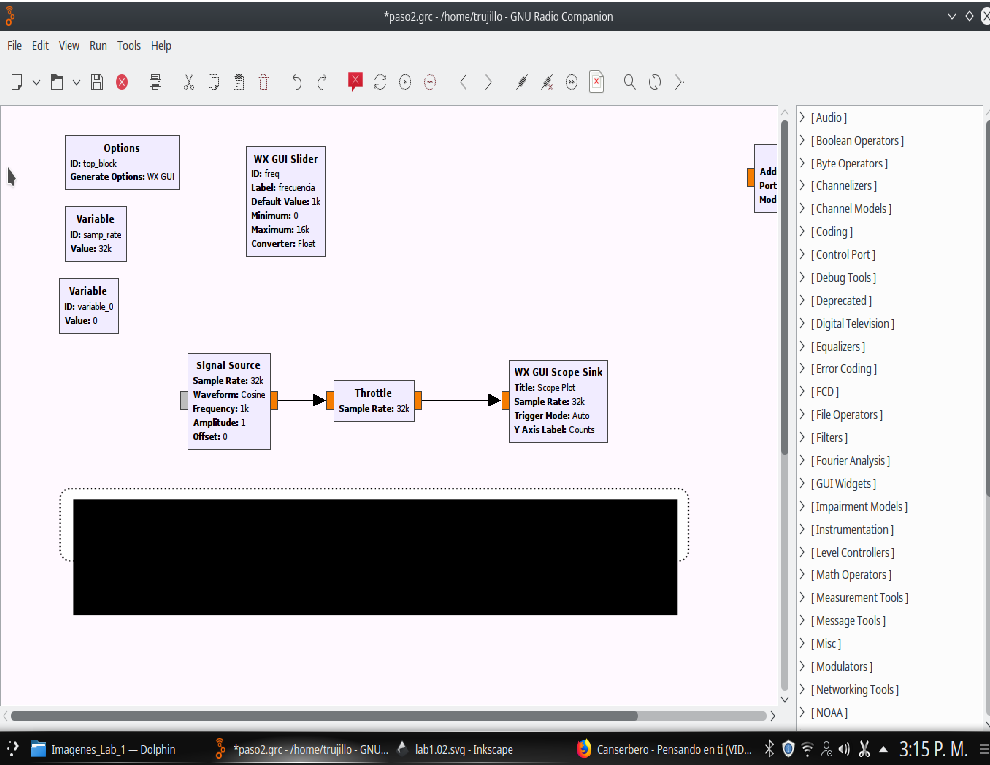
\includegraphics[width=0.9\textwidth]{parte1/lab1/pdf/lab1_2.pdf}
\end{figure}
\end{frame}
%-----------------------------------

\begin{frame}{Primeros pasos }
\begin{figure}[H]
\vspace{-3mm}
\centering
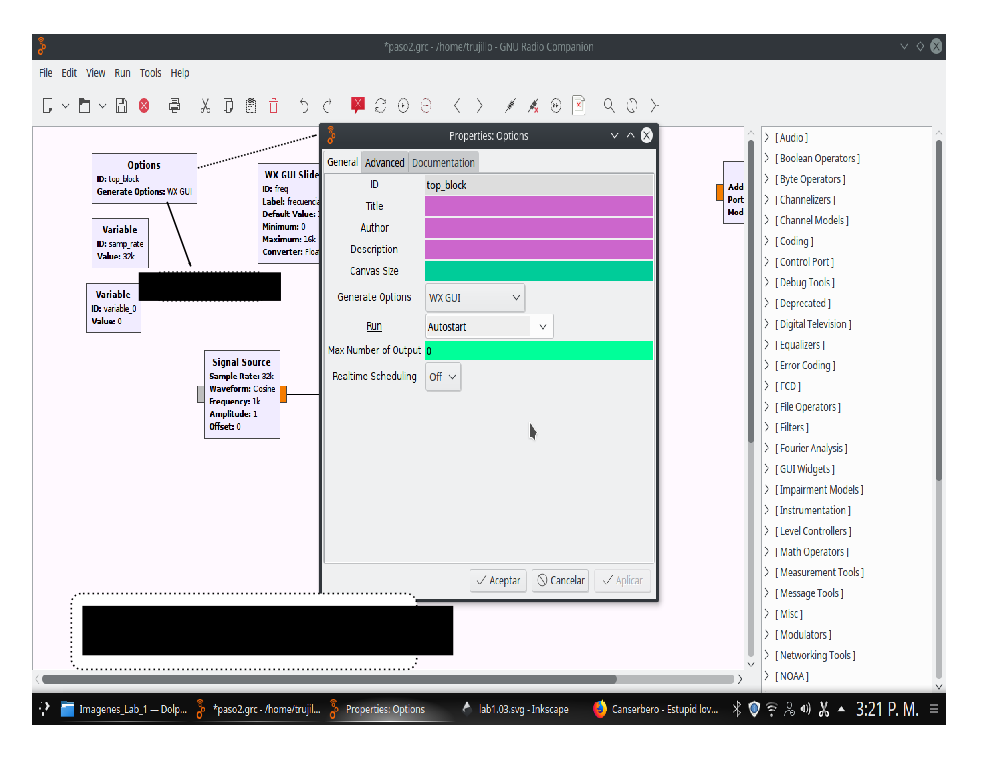
\includegraphics[width=0.9\textwidth]{parte1/lab1/pdf/lab1_3.pdf}
\end{figure}
\end{frame}
%-----------------------------------

\begin{frame}{Primeros pasos }
\begin{figure}[H]
\vspace{-3mm}
\centering
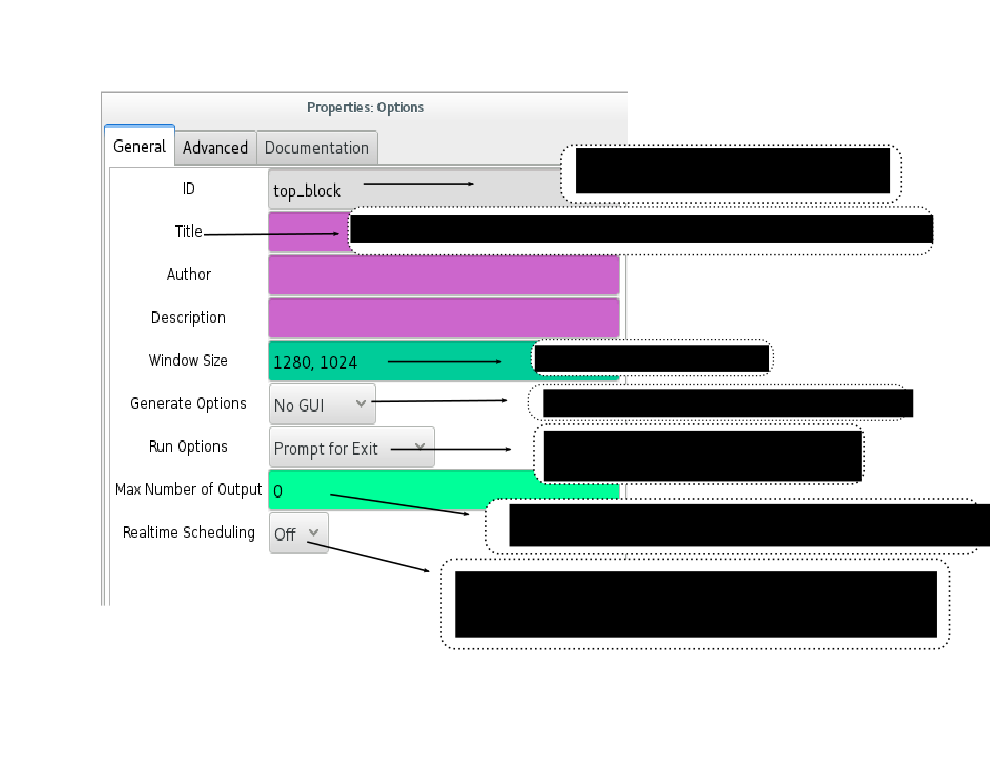
\includegraphics[width=0.9\textwidth]{parte1/lab1/pdf/lab1_4.pdf}
\end{figure}
\end{frame}
%-----------------------------------

\begin{frame}{Primeros pasos }
\begin{figure}[H]
\vspace{-2cm}
\centering
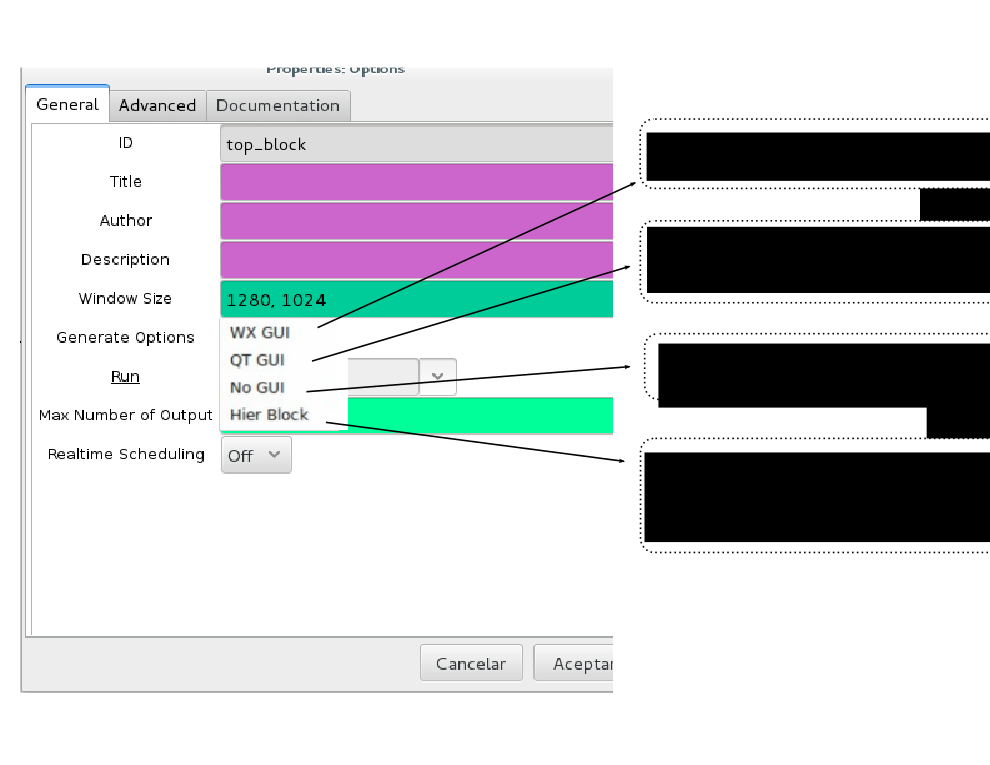
\includegraphics[width=1.1\textwidth]{parte1/lab1/pdf/lab1_5.pdf}
\end{figure}
\end{frame}
%-----------------------------------

\begin{frame}{Primeros pasos }
\begin{figure}[H]
\centering
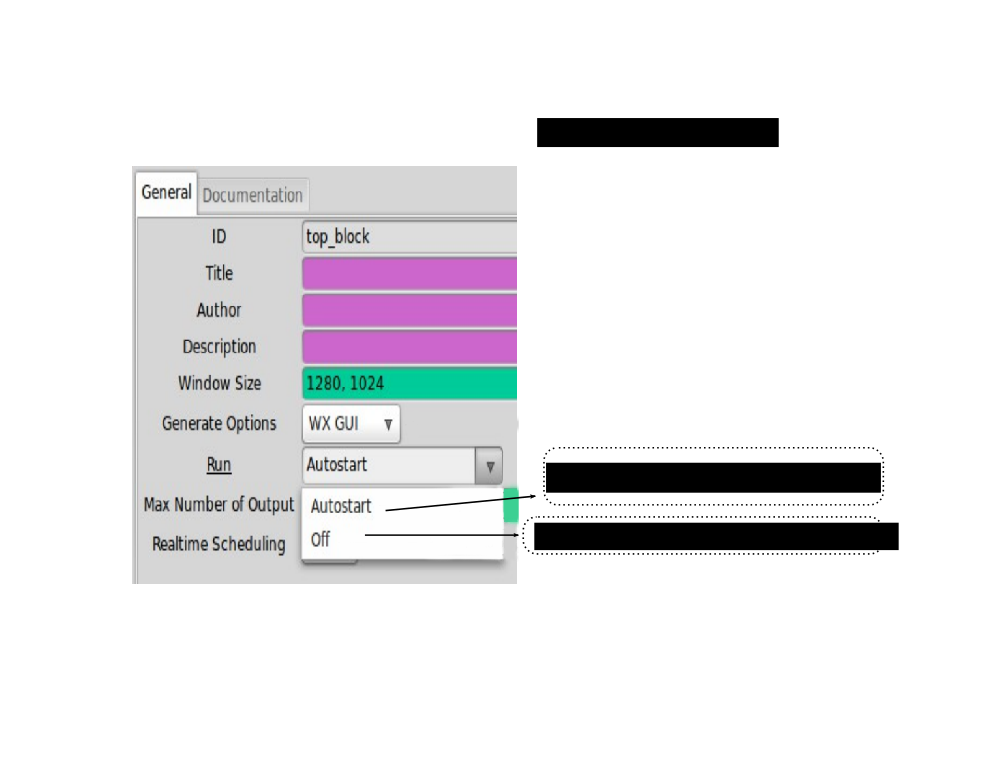
\includegraphics[width=.9\textwidth]{parte1/lab1/pdf/lab1_6.pdf}
\end{figure}
\end{frame}
%-----------------------------------

\begin{frame}{Primeros pasos }
\begin{figure}[H]
\centering
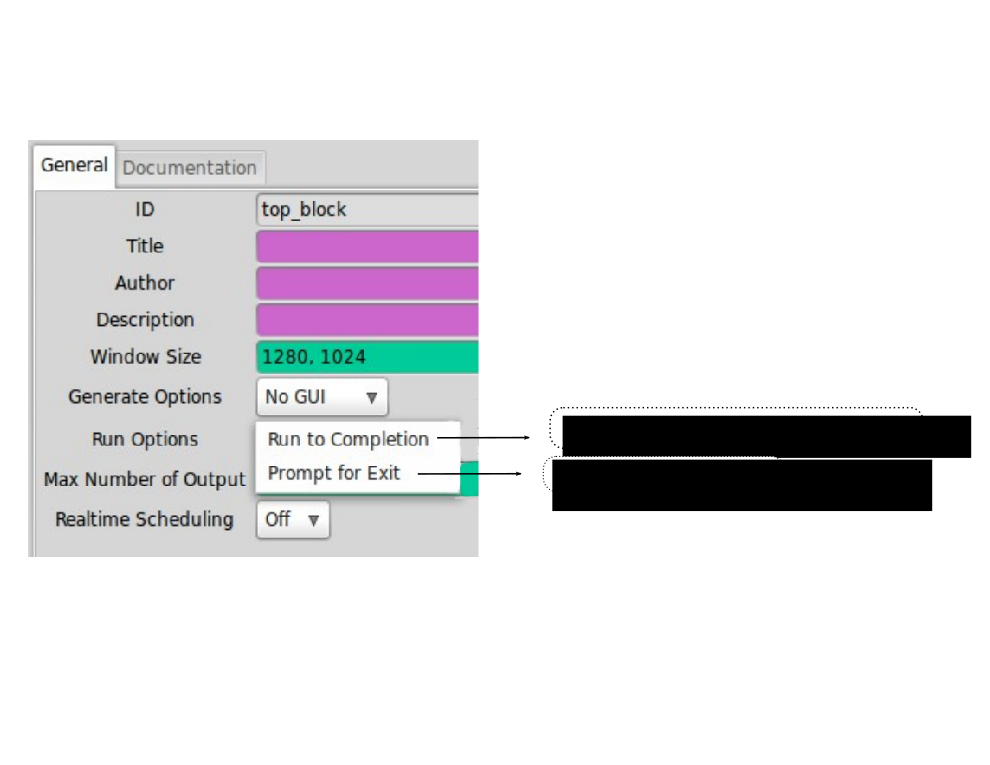
\includegraphics[width=\textwidth]{parte1/lab1/pdf/lab1_7.pdf}
\end{figure}
\end{frame}
%-----------------------------------

\begin{frame}{Primeros pasos }
\begin{figure}[H]
\vspace{-1cm}
\centering
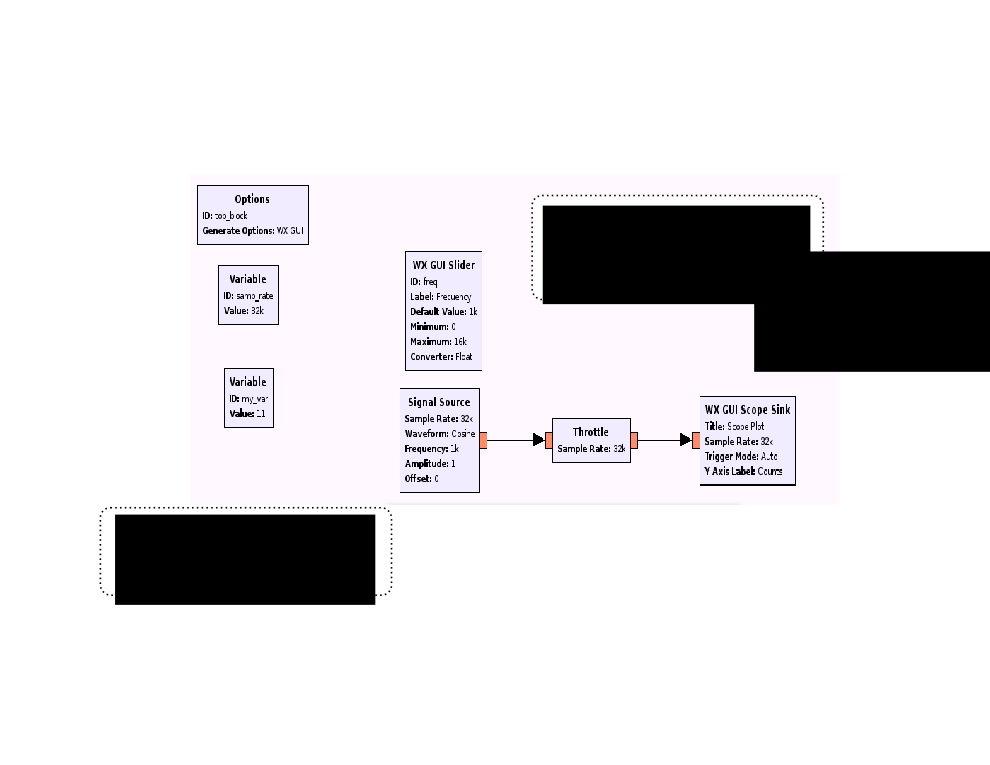
\includegraphics[width=\textwidth]{parte1/lab1/pdf/lab1_8.pdf}
\end{figure}
\end{frame}
%-----------------------------------

\begin{frame}{Primeros pasos }
\begin{figure}[H]
\vspace{-3mm}
\centering
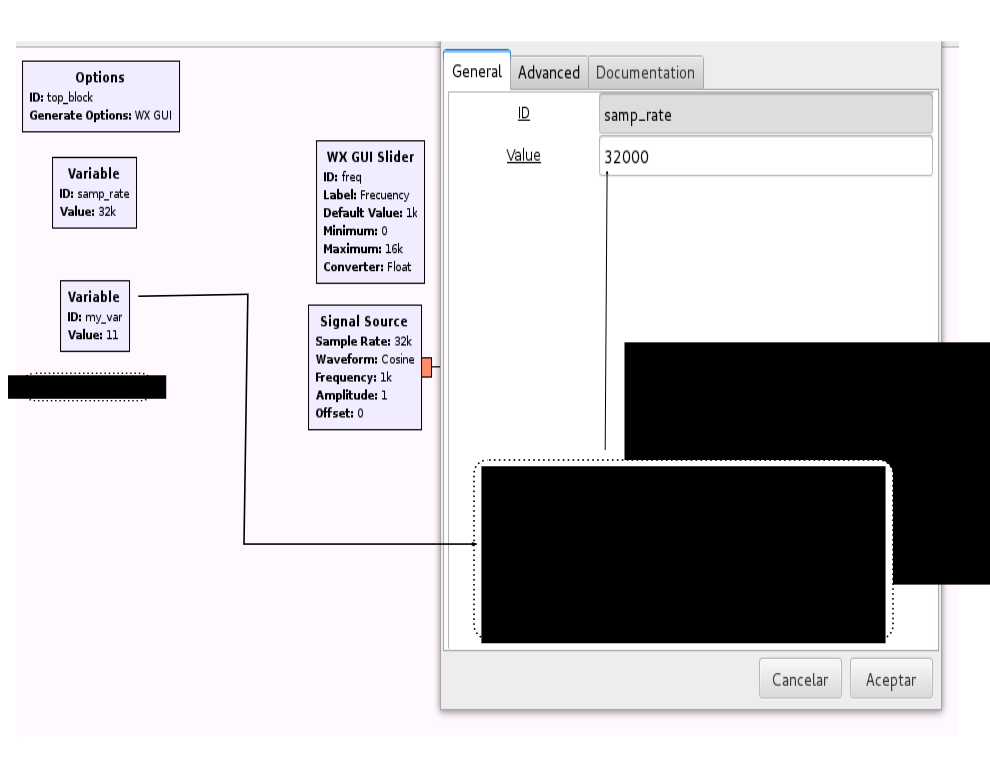
\includegraphics[width=0.85\textwidth]{parte1/lab1/pdf/lab1_9.pdf}
\end{figure}
\end{frame}
%-----------------------------------

\begin{frame}{Primeros pasos }
\begin{figure}[H]
\vspace{-3mm}
\centering
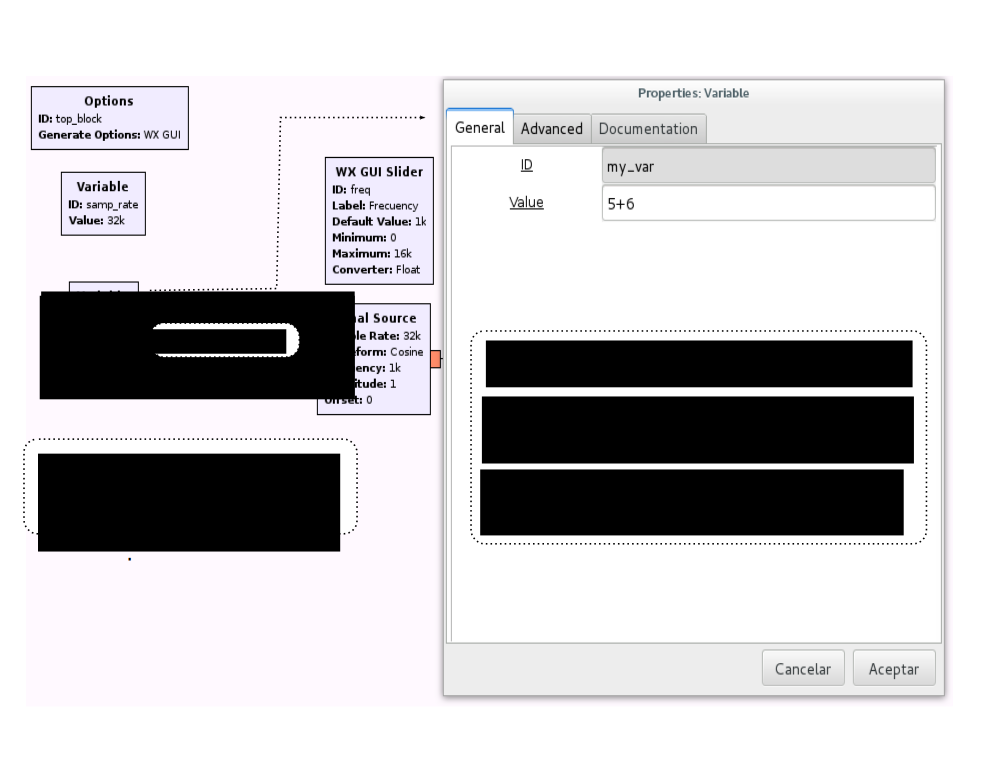
\includegraphics[width=.9\textwidth]{parte1/lab1/pdf/lab1_10.pdf}
\end{figure}
\end{frame}
%-----------------------------------

\begin{frame}{Primeros pasos }
\begin{figure}[H]
\vspace{-3mm}
\centering
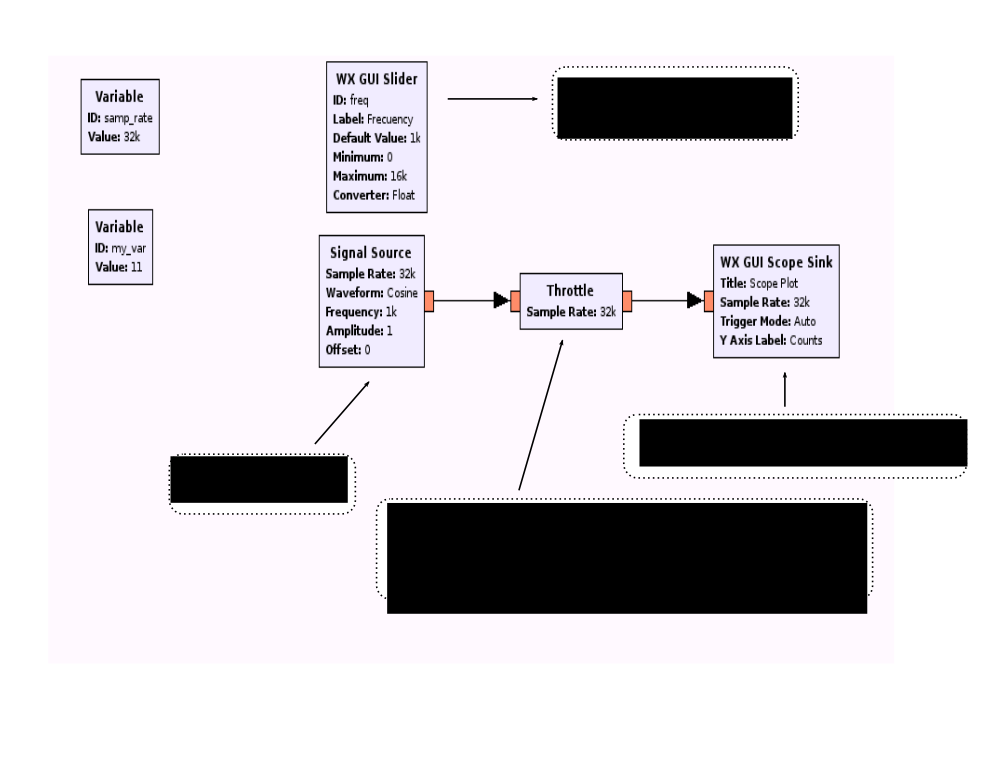
\includegraphics[width=\textwidth]{parte1/lab1/pdf/lab1_11.pdf}
\end{figure}
\end{frame}
%-----------------------------------

\begin{frame}{Primeros pasos }
\begin{figure}[H]
\vspace{-3mm}
\centering
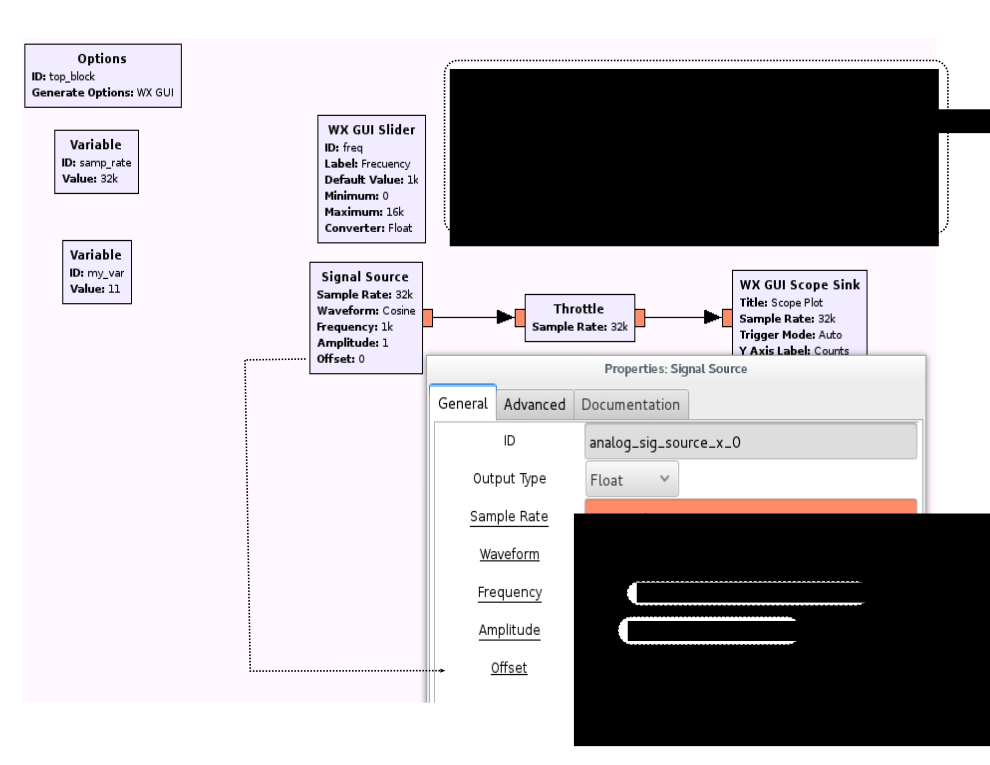
\includegraphics[width=.85\textwidth]{parte1/lab1/pdf/lab1_12.pdf}
\end{figure}
\end{frame}
%-----------------------------------

\begin{frame}{Primeros pasos }
\begin{figure}[H]
\vspace{-3mm}
\centering
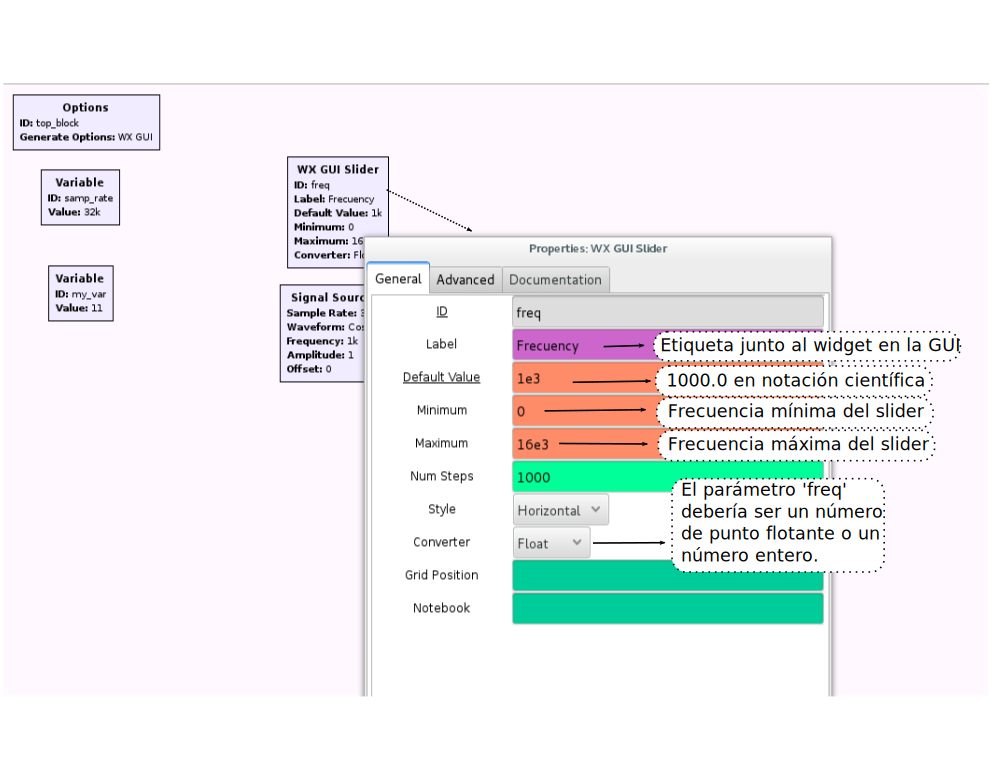
\includegraphics[width=\textwidth]{parte1/lab1/pdf/lab1_13.pdf}
\end{figure}
\end{frame}
%-----------------------------------

\begin{frame}{Primeros pasos }
\begin{figure}[H]
\vspace{-1cm}
\centering
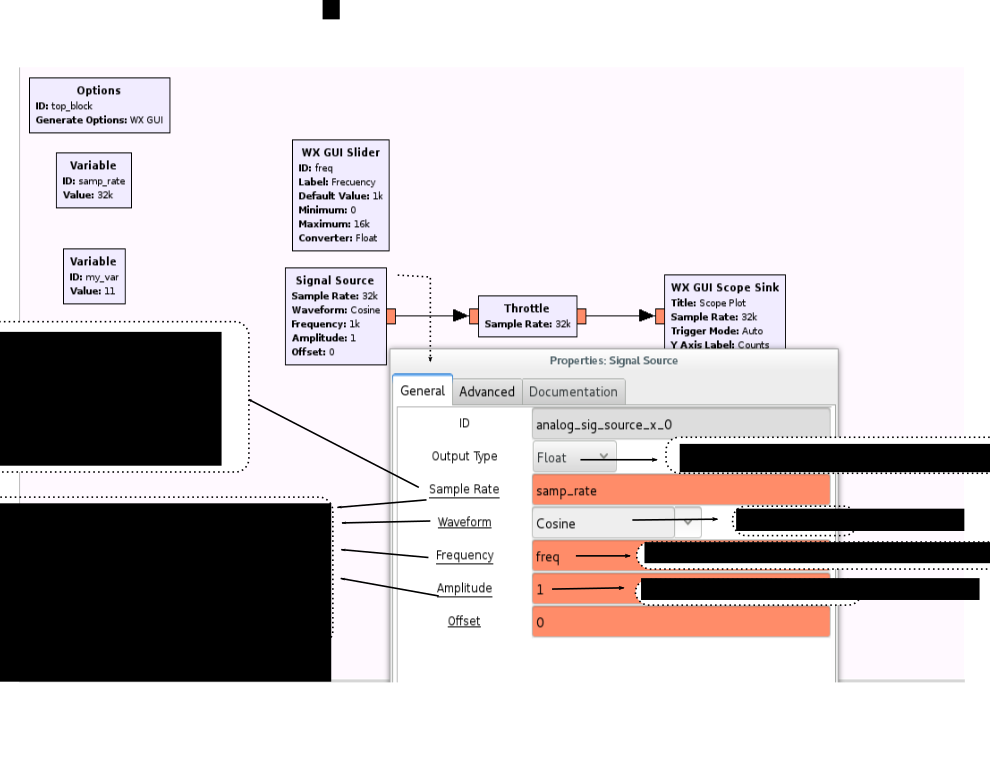
\includegraphics[width=1.05\textwidth]{parte1/lab1/pdf/lab1_14.pdf}
\end{figure}
\end{frame}
%-----------------------------------

\begin{frame}{Primeros pasos }
\begin{figure}[H]
\vspace{-3mm}
\centering
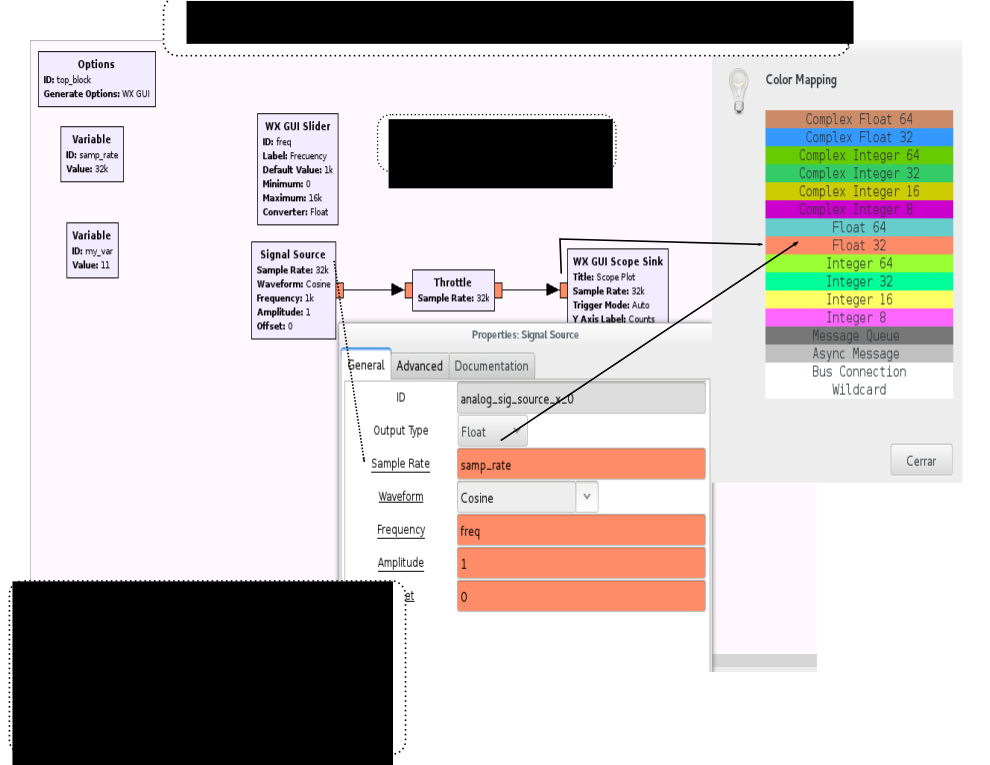
\includegraphics[width=.80\textwidth]{parte1/lab1/pdf/lab1_15.pdf}
\end{figure}
\end{frame}
%-----------------------------------

\begin{frame}{Primeros pasos }
\begin{figure}[H]
\centering
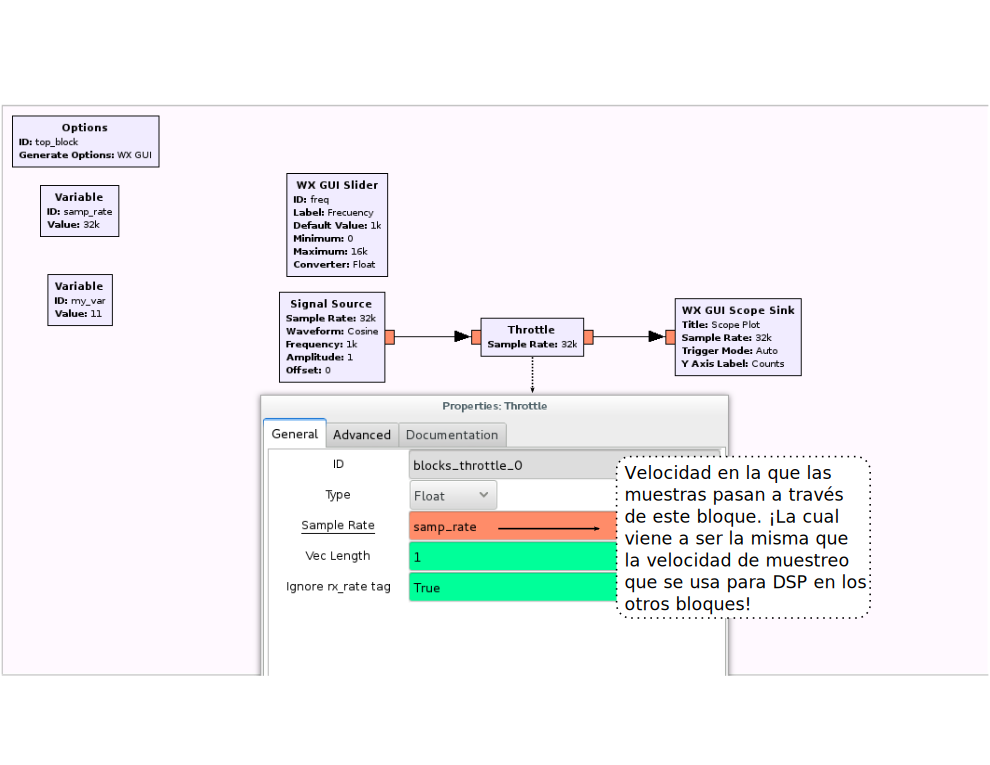
\includegraphics[width=\textwidth]{parte1/lab1/pdf/lab1_16.pdf}
\end{figure}
\end{frame}
%-----------------------------------

\begin{frame}{Primeros pasos }
\begin{figure}[H]
\vspace{-3mm}
\centering
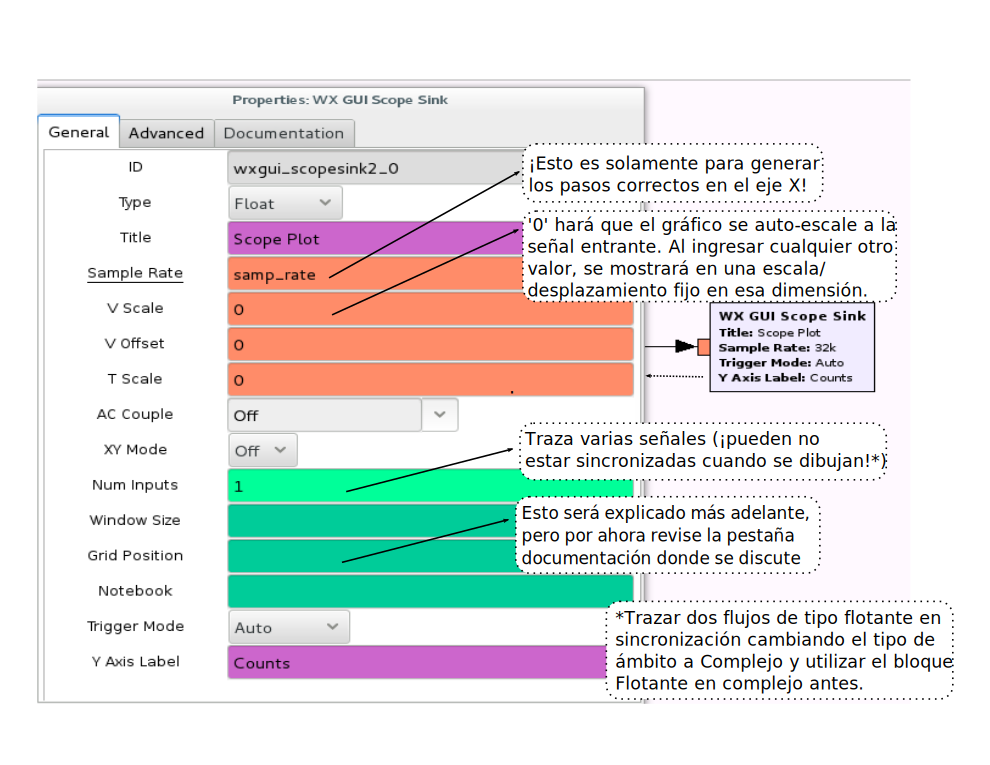
\includegraphics[width=.85\textwidth]{parte1/lab1/pdf/lab1_17.pdf}
\end{figure}
\end{frame}
%-----------------------------------

\begin{frame}{Primeros pasos }
\begin{figure}[H]
\centering
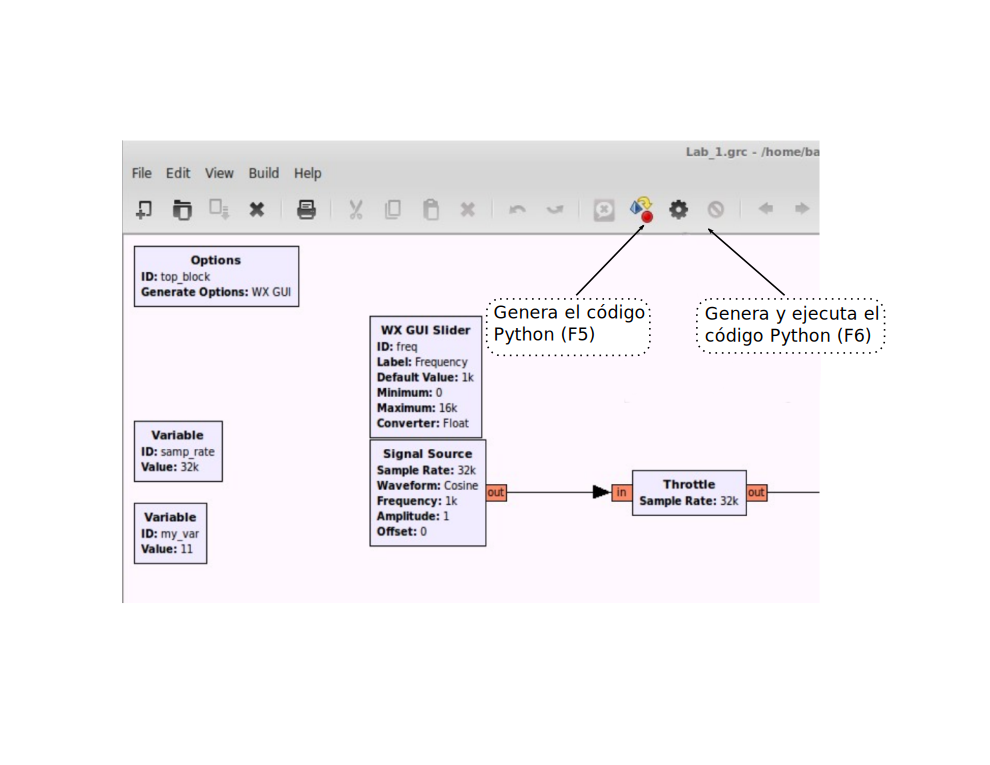
\includegraphics[width=\textwidth]{parte1/lab1/pdf/lab1_18.pdf}
\end{figure}
\end{frame}
%-----------------------------------

\begin{frame}{Primeros pasos }
\begin{figure}[H]
\centering
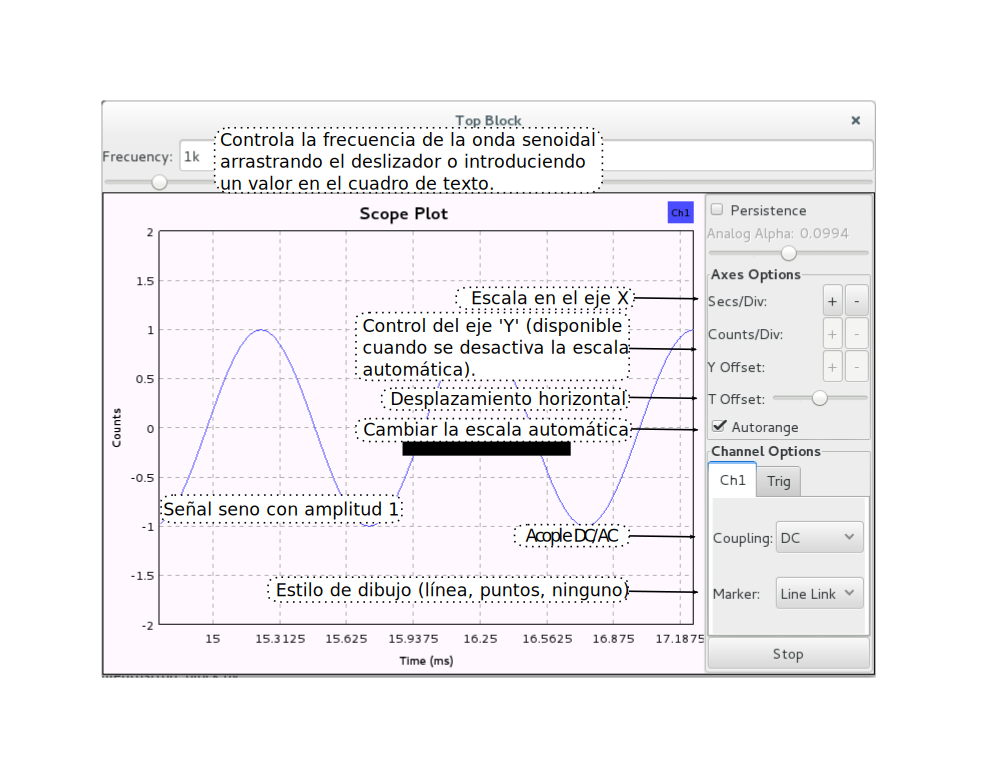
\includegraphics[width=\textwidth, height=0.55\textwidth]{parte1/lab1/pdf/lab1_19.pdf}
\end{figure}
\end{frame}
%-----------------------------------

\begin{frame}{Primeros pasos }
\begin{figure}[H]
\centering
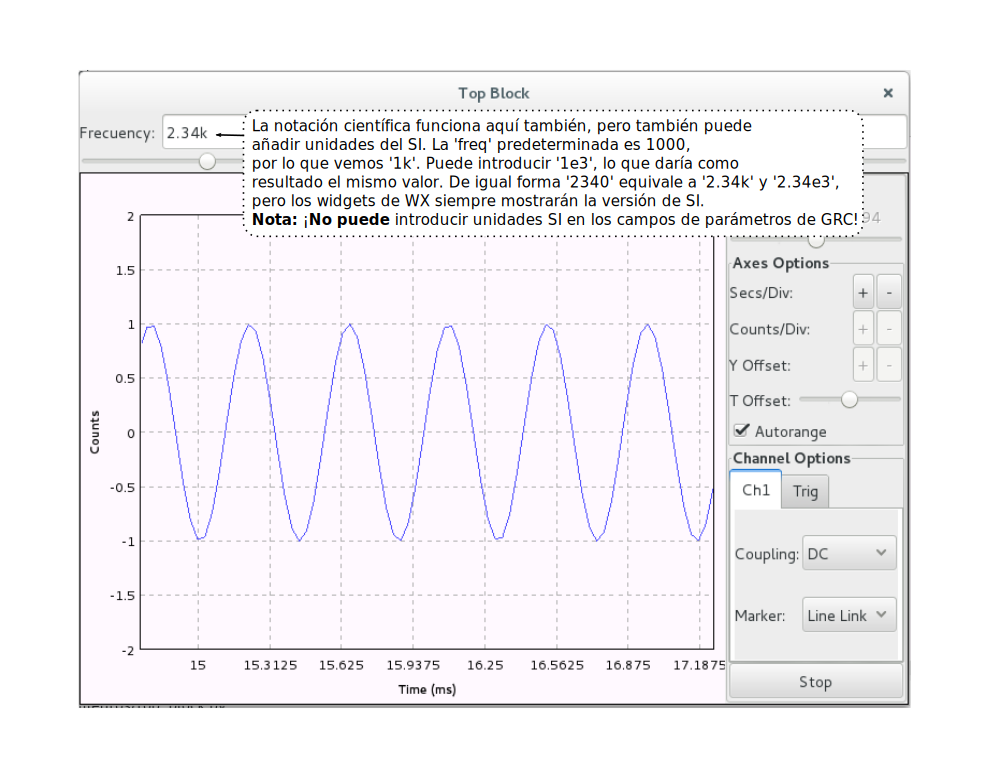
\includegraphics[width=\textwidth, height=0.55\textwidth]{parte1/lab1/pdf/lab1_20.pdf}
\end{figure}
\end{frame}
%-----------------------------------

\begin{frame}{Primeros pasos }
\begin{figure}[H]
\centering
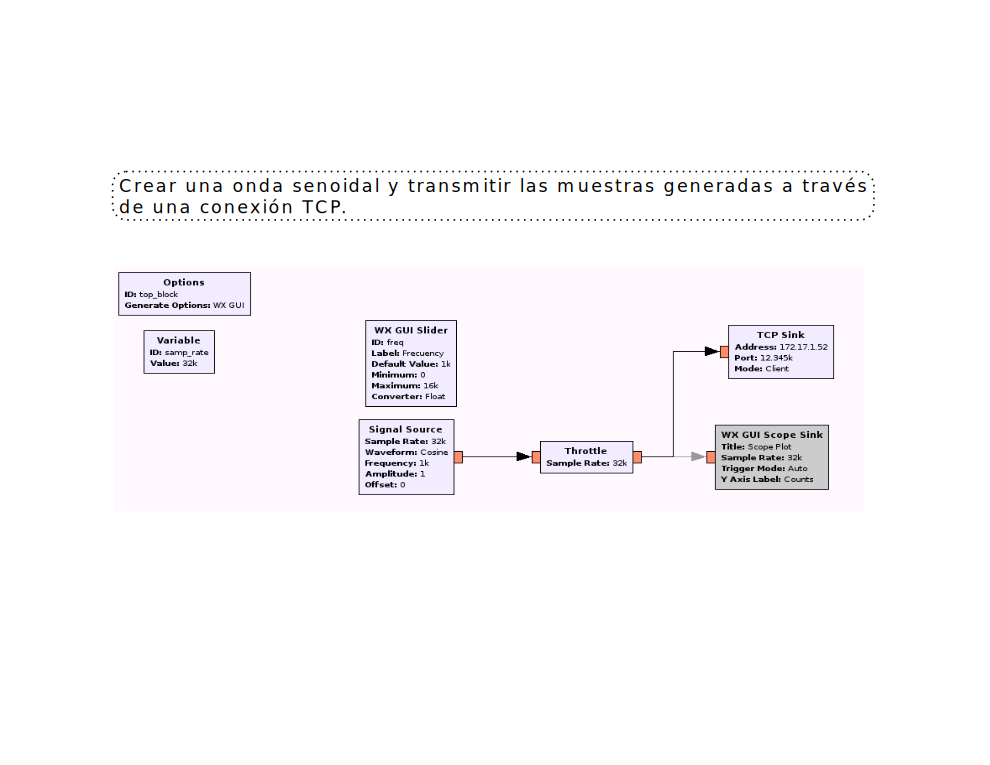
\includegraphics[width=\textwidth]{parte1/lab1/pdf/lab1_21.pdf}
\end{figure}
\end{frame}
%-----------------------------------

\begin{frame}{Primeros pasos }
\begin{figure}[H]
\centering
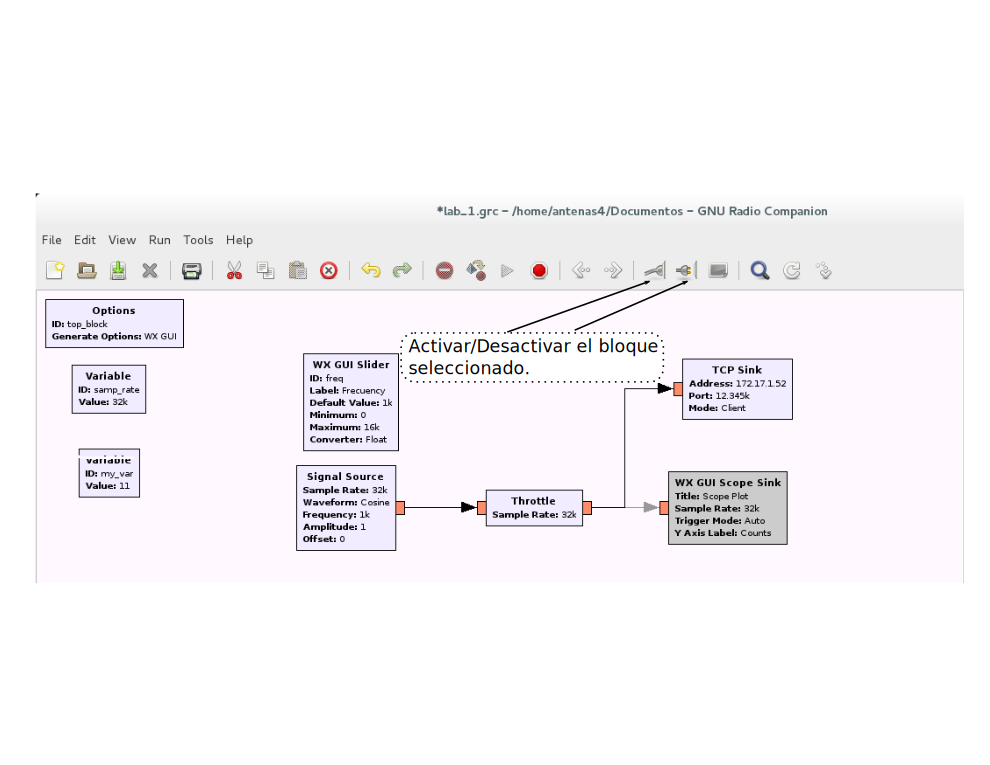
\includegraphics[width=\textwidth]{parte1/lab1/pdf/lab1_22.pdf}
\end{figure}
\end{frame}
%-----------------------------------

\begin{frame}{Primeros pasos }
\begin{figure}[H]
\centering
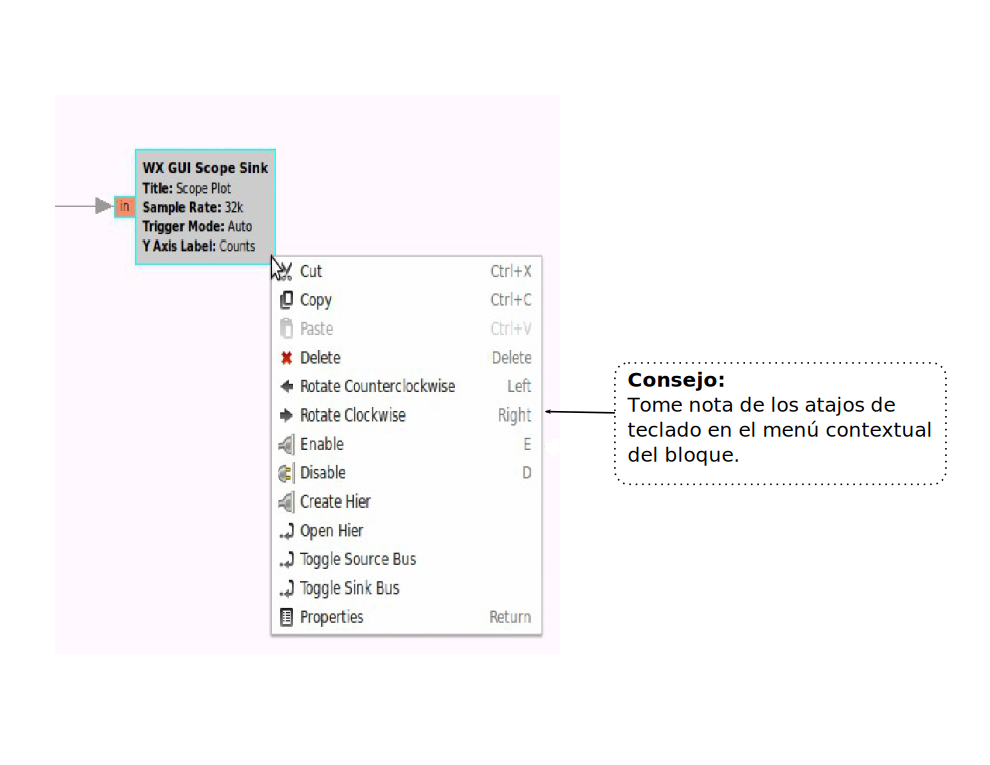
\includegraphics[width=\textwidth, height=0.6\textwidth]{parte1/lab1/pdf/lab1_23.pdf}
\end{figure}
\end{frame}
%-----------------------------------

\begin{frame}{Primeros pasos }
\begin{figure}[H]
\centering
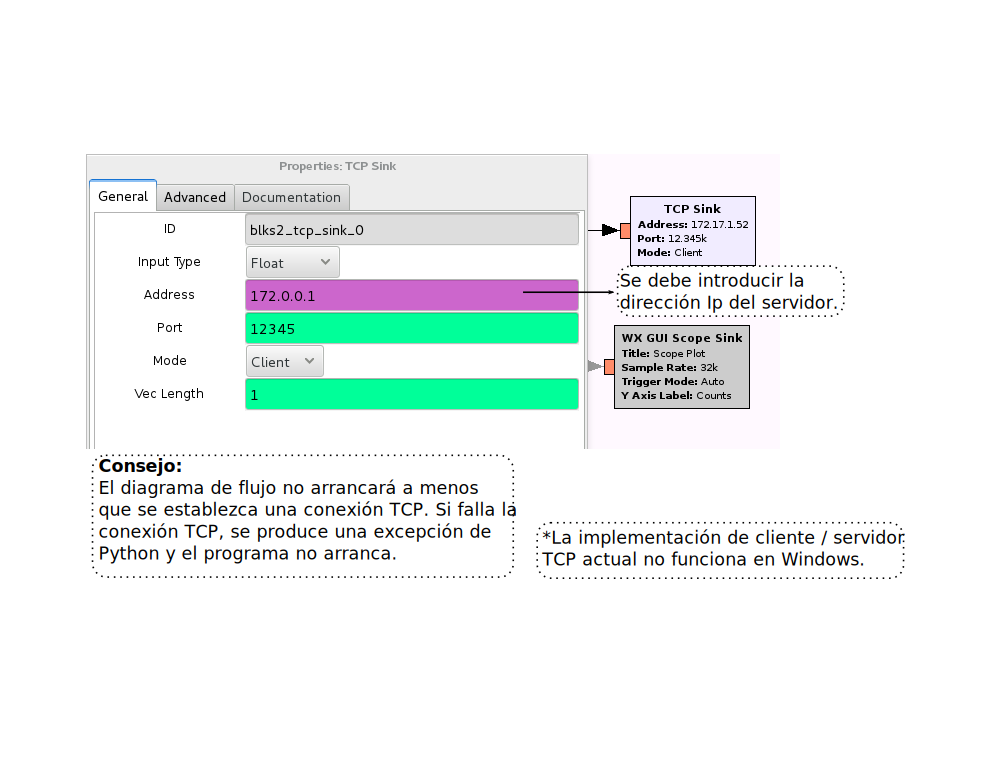
\includegraphics[width=\textwidth]{parte1/lab1/pdf/lab1_24.pdf}
\end{figure}
\end{frame}
%-----------------------------------

\begin{frame}{Primeros pasos }
\begin{figure}[H]
\centering
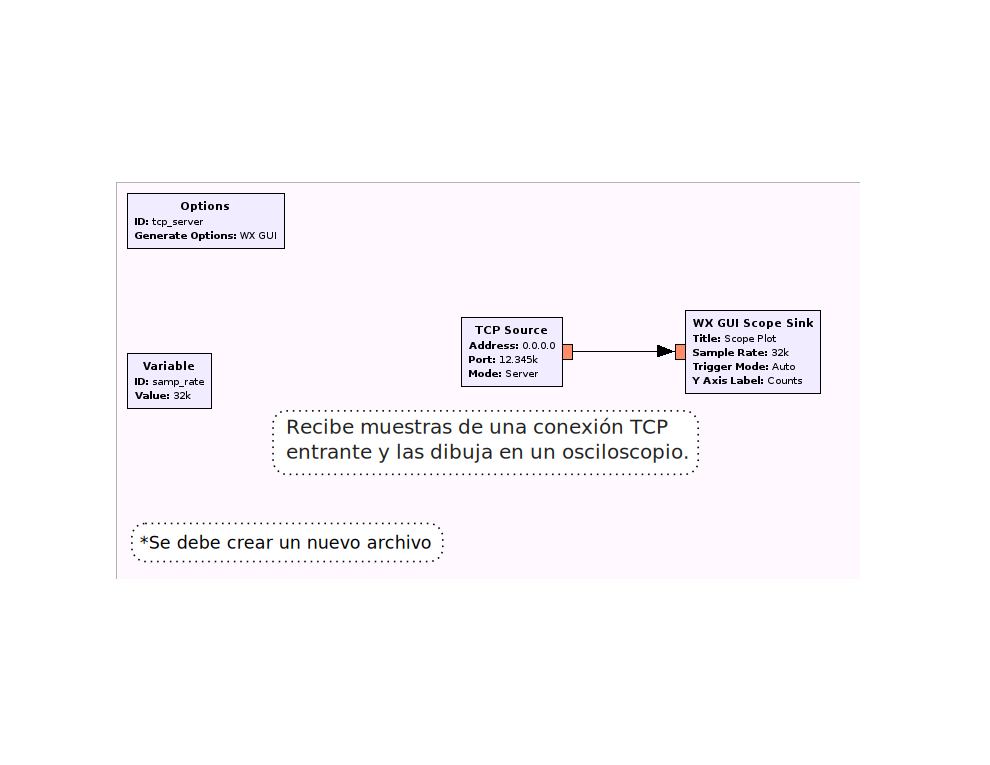
\includegraphics[width=\textwidth]{parte1/lab1/pdf/lab1_25.pdf}
\end{figure}
\end{frame}
%-----------------------------------

\begin{frame}{Primeros pasos }
\begin{figure}[H]
\centering
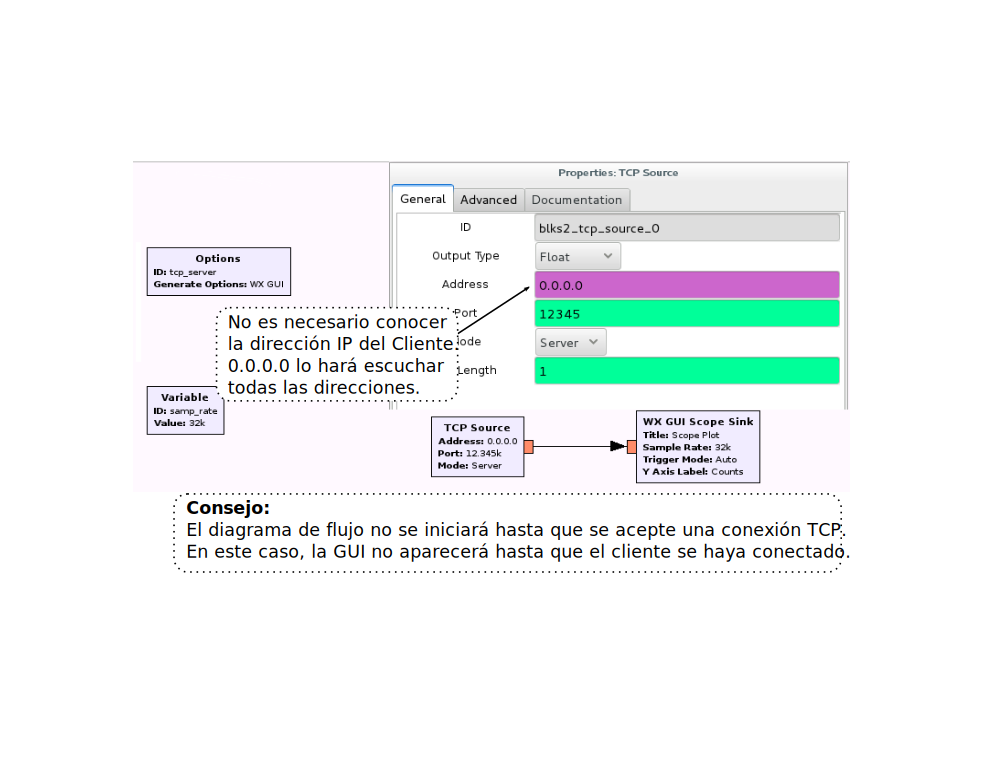
\includegraphics[width=\textwidth]{parte1/lab1/pdf/lab1_26.pdf}
\end{figure}
\end{frame}
%-----------------------------------

\begin{frame}{Primeros pasos }
\begin{figure}[H]
\centering
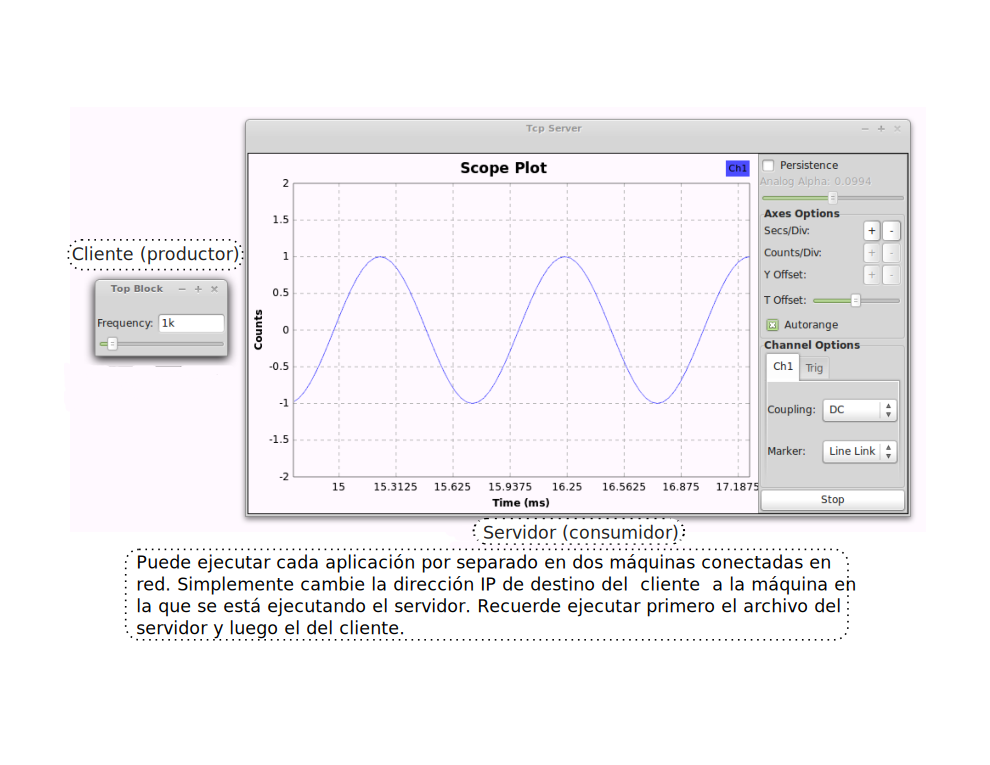
\includegraphics[width=\textwidth, height=0.55\textwidth]{parte1/lab1/pdf/lab1_27.pdf}
\end{figure}
\end{frame}
%-----------------------------------

%///////////////////////////////////////////////////////////////

